\documentclass[conference,a4paper]{IEEEtran}
\IEEEoverridecommandlockouts
% ============================================================
% Paquetes
% ============================================================
\usepackage[utf8]{inputenc}
\usepackage[T1]{fontenc}
\usepackage[spanish,es-tabla]{babel}
\usepackage{amsmath,amssymb,amsfonts}
\usepackage{graphicx}
\usepackage{textcomp}
\usepackage{xcolor}
\usepackage{booktabs}
\usepackage{multirow}
\usepackage{array}
\usepackage{float}
\usepackage{cite}

\graphicspath{{../figs/etapas/}{../chapters/chapter3/Sections/Research Questions/sections/RQ2/img/}}

% Traducción segura de "Index Terms" (no falla si la macro no existe en la instalación)
\makeatletter
\@ifundefined{IEEEkeywordsname}{\newcommand{\IEEEkeywordsname}{Palabras Clave}}{\renewcommand{\IEEEkeywordsname}{Palabras Clave}}
\makeatother

\begin{document}

\title{%
Benefit of Class Balancing Is Metric-Dependent: Feature Selection and Software Defect Prediction Evidence from BugHunter\\[6pt]
{\normalfont\normalsize\itshape(Versión extendida --- título original: ``Feature Selection Beats Class Balancing in Software Defect Prediction: Evidence from BugHunter'')\par}}

% ------------------------------------------------------------------
% Formato de autores IEEE (plantilla oficial):
%   línea 1: Nombre Apellido        <- sin grados académicos (Dr., Ph.D.)
%   línea 2: departamento (cursiva)
%   línea 3: institución (cursiva)
%   línea 4: Ciudad, País
%   línea 5: correo electrónico u ORCID
% ------------------------------------------------------------------
% \and separa los bloques y los distribuye en columnas (3 autores = 3 columnas).
% El nombre del departamento se corta a mano para que las 3 columnas quepan
% lado a lado sin desbordar el ancho de página.
\author{
\IEEEauthorblockN{1\textsuperscript{er} Jordanys Rodríguez Wong}
\IEEEauthorblockA{\textit{Depto. de Ingeniería de} \\
\textit{Sistemas y Computación} \\
\textit{Universidad Católica del Norte} \\
Antofagasta, Chile}
\and
\IEEEauthorblockN{2\textsuperscript{do} Claudio Meneses Villegas}
\IEEEauthorblockA{\textit{Depto. de Ingeniería de} \\
\textit{Sistemas y Computación} \\
\textit{Universidad Católica del Norte} \\
Antofagasta, Chile}
\and
\IEEEauthorblockN{3\textsuperscript{er} Jaime Pavlich-Mariscal}
\IEEEauthorblockA{\textit{Depto. de Ingeniería de} \\
\textit{Sistemas} \\
\textit{Pontificia Universidad Javeriana} \\
Bogotá, Colombia}
}

\maketitle

\begin{abstract}
La predicción de defectos de software enfrenta dos retos persistentes: alta dimensionalidad y desequilibrio de clases. Este trabajo evalúa empíricamente si un preprocesamiento en dos etapas, i.e., selección de características por análisis de relevancia y control de redundancia, seguida de balanceo de clases, mejora la predicción sobre BugHunter, un dataset de 15 proyectos Java con métricas en tres niveles de granularidad (archivo, clase, método). Se aplican Ganancia de Información, Chi-Cuadrado y ReliefF para relevancia; Incertidumbre Simétrica y Semejanza de Coseno para redundancia; ROS, RUS y SMOTE para balanceo; y Random Forest, XGBoost y SVM lineal como clasificadores, totalizando 42.356 ejecuciones. Los resultados muestran que la selección de características reduce la dimensionalidad, con una reducción mediana de 40\,\%, 88\,\% y 50\,\% de las métricas en los niveles de método, clase y archivo, respectivamente, y hasta un 94\,\% en el mejor caso individual, con pérdida de \textit{F-measure} inferior a 0,02 y que las métricas de tamaño de código (CLOC, LOC, LLOC) son los predictores más consistentes en los tres niveles. El hallazgo más relevante concierne al balanceo: aplicado solo al entrenamiento, no mejora el \textit{F-measure} ponderado cuando el conjunto de prueba conserva la distribución real, efecto confirmado con prueba de Wilcoxon pareada y tamaño de efecto de Cliff ($|\delta| < 0{,}15$), pero sí mejora de forma consistente la detección de la clase minoritaria (\textit{F-measure} de la clase \textit{bug} y MCC) en los tres clasificadores, un beneficio que la métrica agregada enmascara. Entrenar por proyecto individual supera sistemáticamente al entrenamiento con el conjunto unificado en los tres clasificadores. Estos resultados indican que la conclusión sobre la utilidad del balanceo de clases depende críticamente de la métrica de evaluación empleada, una advertencia metodológica relevante para la predicción de defectos de software en general.
\end{abstract}

\begin{IEEEkeywords}
predicción de defectos de software, selección de características, desequilibrio de clases, BugHunter, Random Forest, MCC, reconocimiento de patrones
\end{IEEEkeywords}

\section{Introducción}

El uso de sistemas de software en la vida cotidiana crece exponencialmente a medida que se integran en más ámbitos, lo que obliga a los equipos de desarrollo a mantener altos estándares de calidad en cada fase del ciclo de vida. Las pruebas de software son una de las fases más críticas, ya que las fallas no detectadas pueden derivar en transacciones defectuosas, interrupciones de servicio y fallas en cascada sobre sistemas dependientes \cite{singh2024,ferenc2020}. La Predicción de Fallas de Software (PFS) busca anticipar estos problemas identificando, antes de la fase de pruebas, los elementos de código con mayor probabilidad de contener errores.

Durante años, el principal obstáculo de la PFS fue la escasez de conjuntos de datos públicos, lo que dificultaba comparar métodos entre estudios. Repositorios como PROMISE \cite{promise2005}, inspirados en el repositorio de aprendizaje automático de la UCI \cite{uci1987}, y conjuntos como NASA, SOFTLAB, ReLink, AEEEM y Eclipse ayudaron a paliar este problema, aunque la mayoría se limita a métricas tradicionales de tamaño y complejidad ciclomática capturadas en una o pocas versiones de lanzamiento. Ferenc et al. \cite{ferenc2020} propusieron un enfoque distinto: capturar el estado del código inmediatamente antes y después de cada corrección de error en 15 proyectos Java de GitHub, dando origen al conjunto de datos BugHunter, que registra métricas en tres niveles de granularidad (archivo, clase y método).

La calidad de estos conjuntos de datos condiciona directamente el desempeño de los modelos de predicción \cite{rathi2023}. Entre los problemas más señalados en la literatura están la alta dimensionalidad, producto de características poco relevantes o redundantes, y el desequilibrio de clases, dado que las instancias sin errores superan ampliamente a las instancias con errores \cite{tantithamthavorn2020}. Este trabajo aborda ambos problemas sobre BugHunter mediante dos técnicas complementarias: (i) selección de características en dos etapas, combinando análisis de relevancia y control de redundancia, y (ii) balanceo de clases sobre el conjunto de entrenamiento mediante \textit{Random Over-Sampling} (ROS), \textit{Random Under-Sampling} (RUS) y \textit{Synthetic Minority Over-sampling Technique} (SMOTE).

Como línea base, se replican los resultados originales de \cite{ferenc2020} empleando el clasificador Random Forest en Weka sobre BugHunter sin procesar. A partir de esa línea base, este artículo busca responder cinco preguntas de investigación:

\begin{itemize}
\item \textbf{RQ1.} \textquestiondown{}El análisis de relevancia y el control de redundancia de características mejoran la identificación de errores basada en métricas de código?
\item \textbf{RQ2.} \textquestiondown{}Qué métricas de código son mejores predictoras de errores y en qué nivel de granularidad ofrecen mejores resultados?
\item \textbf{RQ3.} \textquestiondown{}Cómo influye la variación de los parámetros de los algoritmos de relevancia y redundancia en los resultados de clasificación?
\item \textbf{RQ4.} \textquestiondown{}Cómo influyen los algoritmos de balanceo de clases ROS, RUS y SMOTE en los resultados de los clasificadores?
\item \textbf{RQ5.} \textquestiondown{}Qué diferencias existen entre entrenar con el conjunto unificado de proyectos y entrenar con cada proyecto por separado?
\end{itemize}

La principal contribución de este trabajo es una evaluación experimental exhaustiva, con 13.916 ejecuciones de Random Forest complementadas por un análisis de sensibilidad de 28.440 ejecuciones adicionales con XGBoost y SVM lineal, de la combinación de selección de características y balanceo de clases sobre BugHunter, que identifica las métricas de código más relevantes, cuantifica el efecto real del balanceo de clases cuando el conjunto de prueba conserva su distribución original ---incluido su efecto sobre las métricas por clase---, y compara el entrenamiento por proyecto individual frente al entrenamiento con un conjunto unificado. Esta versión extendida, además, explicita el orden de las etapas de preprocesamiento respecto de la partición entrenamiento/prueba, incorpora advertencias adicionales sobre sesgos de selección post-hoc en RQ1 y RQ2, y declara explícitamente como trabajo futuro la validación mediante un esquema de selección de características anidado y validación cruzada repetida (Secciones \ref{sec:metodologia}, \ref{sec:amenazas} y \ref{sec:conclusiones}). El resto del artículo se organiza así: la Sección II resume trabajos relacionados; la Sección III describe el conjunto de datos y la metodología; la Sección IV presenta los resultados experimentales organizados por pregunta de investigación; la Sección V discute los hallazgos y sus amenazas a la validez; y la Sección VI concluye con el trabajo futuro.

\section{Trabajos Relacionados}

BugHunter \cite{ferenc2020} se diferencia de conjuntos de datos tradicionales como PROMISE o Eclipse \cite{promise2005} porque captura métricas de código en el instante más cercano posible a la introducción y corrección de un error, en lugar de comparar versiones de lanzamiento completas. Las métricas se extraen con la herramienta OpenStaticAnalyzer \cite{osa2004} en tres niveles (archivo, clase, método), lo que permite estudiar en qué nivel de granularidad las métricas de código son más informativas. Singh y Thankachan \cite{singh2021survey} ofrecen una revisión amplia de los marcos de aprendizaje automático aplicados a la PFS, mientras que Li et al. \cite{li2018} sintetizan el estado del arte hasta 2018, señalando el desequilibrio de clases y la alta dimensionalidad como los principales desafíos abiertos.

Liu et al. \cite{liu2015} y Chen et al. \cite{chen2013} propusieron el marco de preprocesamiento en dos etapas que se adopta en este trabajo: primero un análisis de relevancia (Ganancia de Información, Chi-Cuadrado, ReliefF) y luego un control de redundancia basado en agrupamiento por umbral (\textit{Neighbor-based Threshold Clustering}, NTC), usando Incertidumbre Simétrica \cite{yu2003} o Semejanza de Coseno como medidas de similitud entre características. Cabe notar que estos trabajos, al igual que el presente estudio en su diseño original, calculan la selección de características sobre el conjunto completo antes de particionar entrenamiento y prueba, una práctica común en la literatura de selección de características para PFS cuya implicancia se discute en las Secciones \ref{sec:seleccion} y \ref{sec:amenazas} de esta versión extendida. Sobre el desequilibrio de clases, Tantithamthavorn et al. \cite{tantithamthavorn2020} muestran que el efecto de las técnicas de rebalanceo depende fuertemente del contexto experimental, mientras que Rathi et al. \cite{rathi2023} y Hossen et al. \cite{hossen2020} reportan mejoras al combinar muestreo y selección de características sobre proyectos de PROMISE. A diferencia de estos últimos, el presente trabajo evalúa dicha combinación sobre BugHunter, comparando explícitamente los tres niveles de granularidad y contrastando el entrenamiento por proyecto individual frente al conjunto unificado, un análisis (RQ5) no cubierto en los estudios anteriores.

Una línea de trabajo más reciente sustituye las métricas de código por representaciones profundas del código fuente. {\v S}iki\'c et al. \cite{sikic2022} aplican redes neuronales de grafos (GNN) sobre representaciones derivadas del árbol de sintaxis abstracta (AST) para predecir defectos, Zhou et al. \cite{zhou2022} combinan la semántica interna de cada archivo (CNN sobre el AST) con la estructura de dependencias entre clases (GCN), y SeDPGK \cite{liu2024sedpgk} extiende esta ruta al escenario semisupervisado mediante destilación de conocimiento sobre grafos de dependencias. Pornprasit y Tantithamthavorn \cite{pornprasit2023} proponen DeepLineDP, un modelo jerárquico de aprendizaje profundo que localiza defectos a nivel de línea, mientras que Jiang et al. \cite{jiang2024} muestran que una codificación conjunta semántico-sintáctica del AST mejora la transferencia entre proyectos, aunque la heterogeneidad de distribuciones sigue siendo el principal obstáculo. En paralelo, los modelos preentrenados de código se han incorporado a la predicción \textit{just-in-time}: Guo et al. \cite{guo2023} reportan mejoras consistentes con seis \textit{backbones} preentrenados ---donde el balance de los datos de entrenamiento resulta determinante en escenarios de pocos datos---, y el benchmark ReDef \cite{nam2026} muestra que la calidad de las etiquetas condiciona las conclusiones sobre estos modelos, en línea con la motivación de calidad de datos de BugHunter. Las revisiones sistemáticas de Giray et al. \cite{giray2023} y de Stradowski y Madeyski \cite{stradowski2023} coinciden, no obstante, en que estos modelos incrementan considerablemente el costo computacional sin superar de forma consistente a los clasificadores clásicos entrenados sobre métricas tabulares, y señalan la brecha aún abierta entre esta investigación y su adopción industrial. Más recientemente, los modelos de lenguaje de gran escala (LLM) han abierto una nueva agenda de investigación en ingeniería de software \cite{hou2024,fan2023} que incluye la detección de defectos, cuyo estado del arte sintetizan Chen et al. \cite{chen2026llm}. Estos enfoques requieren acceso al código fuente completo y recursos de cómputo considerables; el enfoque de este trabajo ---métricas estáticas tabulares con selección de características y clasificadores clásicos--- conserva un costo bajo y mayor interpretabilidad, y aporta líneas base rigurosas contra las cuales evaluar si las representaciones profundas ofrecen mejoras reales sobre conjuntos como BugHunter.

\section{Conjunto de Datos y Metodología}
\label{sec:metodologia}

\subsection{BugHunter}

BugHunter \cite{ferenc2020} es un conjunto de datos de errores construido automáticamente a partir de 15 proyectos Java alojados en GitHub, seleccionados por su tamaño, dominio y cantidad de errores reportados. A diferencia de los conjuntos de datos tradicionales, que caracterizan todos los elementos de código de una versión de lanzamiento, BugHunter captura el estado de cada elemento de código (archivo, clase o método) justo antes de que se le detecte un error y justo después de su corrección, e ignora los elementos nunca afectados por errores. Las métricas fueron extraídas con OpenStaticAnalyzer \cite{osa2004} e incluyen métricas de tamaño, complejidad, cohesión, acoplamiento, clonación de código y violaciones de reglas de codificación (\textit{code smells}). El conjunto de datos original expone 72 métricas a nivel de método, 92 a nivel de clase y 6 a nivel de archivo por proyecto, además de un conjunto ``All'' por cada nivel que une los 15 proyectos.

La distribución de clases, calculada sobre los 45 conjuntos proyecto-nivel tras binarizar el atributo \textit{Number of Bugs}, se resume en la Tabla \ref{tab:desbalance}. El desequilibrio de BugHunter es moderado si se compara con los conjuntos clásicos de PFS ---como NASA o PROMISE, donde la clase con error suele representar menos del 10\,\% de las instancias~\cite{tantithamthavorn2020}---: la mediana de instancias \textit{bug} entre los 15 proyectos es del 28,1\,\% a nivel de método, 41,1\,\% a nivel de clase y 42,7\,\% a nivel de archivo, y en tres proyectos (\textit{hazelcast}, \textit{MapDB} y \textit{elasticsearch}) la clase \textit{bug} llega a ser mayoritaria a nivel de archivo. Esta característica es consecuencia directa del diseño de BugHunter, que solo incluye elementos de código efectivamente afectados por errores, y acota el sesgo de las métricas agregadas hacia la clase mayoritaria (Sección \ref{sec:amenazas}). El caso más desequilibrado es \textit{oryx} (razón no-bug:bug de 7,6:1 a nivel de método), lo que debe tenerse presente al interpretar su desempeño, el más alto del estudio.

\begin{table}[H]
\caption{Proporción de instancias con error (\textit{bug}) por nivel de granularidad, sobre los 15 proyectos individuales}
\label{tab:desbalance}
\centering
\resizebox{\columnwidth}{!}{%
\begin{tabular}{lccccc}
\toprule
Nivel & Mediana & Mín. (proyecto) & Máx. (proyecto) & ``All'' & Razón mediana \\
      & \% bug  &                 &                 & \% bug  & no-bug:bug \\
\midrule
Método  & 28,1 & 11,7 (\textit{oryx}) & 42,2 (\textit{hazelcast}) & 37,0 & 2,6:1 \\
Clase   & 41,1 & 12,5 (\textit{oryx}) & 53,0 (\textit{hazelcast}) & 48,6 & 1,4:1 \\
Archivo & 42,7 & 13,2 (\textit{oryx}) & 55,2 (\textit{hazelcast}) & 50,7 & 1,3:1 \\
\bottomrule
\end{tabular}}
\end{table}

\subsection{Selección de características en dos etapas}
\label{sec:seleccion}

Siguiendo el marco propuesto por Liu et al. \cite{liu2015}, la selección de características se ejecuta en dos etapas.

\textit{Análisis de relevancia.} Se calcula la importancia de cada característica mediante tres algoritmos: Ganancia de Información (IG), Chi-Cuadrado (CS) y ReliefF (RF). La Ganancia de Información se define como la reducción de entropía al dividir el conjunto de datos según una característica,
\begin{equation}
H = -\sum_{x} p(x)\log_{2}p(x),
\label{eq:entropia}
\end{equation}
donde $p(x)$ es la probabilidad de que una instancia pertenezca a la clase $x$. El estadístico Chi-Cuadrado compara la distribución observada de una característica con la esperada bajo independencia respecto a la clase,
\begin{equation}
\chi^{2} = \sum \frac{(O-E)^{2}}{E}.
\label{eq:chisqr}
\end{equation}
ReliefF, en cambio, actualiza el peso $W[A]$ de cada característica $A$ muestreando instancias al azar y comparándolas con su vecino más cercano de la misma clase (\textit{hit}, $H$) y de la clase contraria (\textit{miss}, $M$),
\begin{equation}
W[A] = W[A] - \frac{\mathrm{diff}(A,R,H)}{m} + \frac{\mathrm{diff}(A,R,M)}{m},
\label{eq:relief}
\end{equation}
donde $R$ es la instancia muestreada, $\mathrm{diff}(\cdot)$ la diferencia normalizada en la característica $A$ y $m$ el número de muestreos. En cada caso se conservan las $k$ características cuyo ranking supera un umbral relativo (\textit{Rank} $\in \{0{,}5, 0{,}7, 0{,}9\}$).

\textit{Control de redundancia.} Sobre el subconjunto resultante se aplica el algoritmo de agrupamiento por umbral NTC \cite{liu2015}, que construye un grafo de vecino más cercano entre características y descarta aquellas cuya similitud con otra característica ya seleccionada supera un umbral $\beta \in \{0{,}5, 0{,}7, 0{,}9\}$. La similitud se mide con Incertidumbre Simétrica (SU),
\begin{equation}
SU(X,Y) = 2 \times \frac{I(X;Y)}{H(X)+H(Y)},
\label{eq:su}
\end{equation}
donde $I(X;Y)$ es la información mutua entre las dos características \cite{yu2003}, o con Semejanza de Coseno (COS) entre los vectores de valores de dos características. La combinación de los tres algoritmos de relevancia con las dos medidas de redundancia produce seis esquemas de selección: IG\_SU, CS\_SU, RF\_SU, IG\_COS, CS\_COS y RF\_COS.

\textit{Precisión sobre el orden de las etapas respecto de la partición entrenamiento/prueba.} El análisis de relevancia y el control de redundancia descritos en esta sección se calculan sobre el conjunto proyecto-nivel completo, es decir, antes de la partición en entrenamiento y prueba descrita en la Sección \ref{sec:diseno}; el balanceo de clases (Sección \ref{sec:balanceo}), en cambio, se aplica exclusivamente dentro del conjunto de entrenamiento resultante. Dado que los tres algoritmos de relevancia (IG, CS, RF) utilizan la etiqueta de clase de cada instancia, este orden introduce un riesgo de sesgo de selección (\textit{selection bias}): el subconjunto de características elegido puede estar influido por patrones presentes en instancias que posteriormente integrarán el conjunto de prueba \cite{ambroise2002,cawley2010}. Este riesgo afecta únicamente la elección estructural de qué columnas conservar, y no los parámetros del clasificador, que se ajustan exclusivamente sobre el conjunto de entrenamiento resultante de dicha selección (Sección \ref{sec:diseno}). La magnitud de este riesgo se discute en la Sección \ref{sec:amenazas}, y su corrección mediante un esquema de selección anidado, recalculado de forma independiente dentro de cada partición de entrenamiento, se declara como trabajo futuro (Sección \ref{sec:conclusiones}).

\subsection{Balanceo de clases}
\label{sec:balanceo}

Sobre el conjunto de entrenamiento resultante de la selección de características se aplican, de forma independiente, tres técnicas de remuestreo \cite{junsomboon2017,hossen2020}: \textit{Random Under-Sampling} (RUS), que elimina aleatoriamente instancias de la clase mayoritaria; \textit{Random Over-Sampling} (ROS), que duplica aleatoriamente instancias de la clase minoritaria; y SMOTE, que genera instancias sintéticas de la clase minoritaria interpolando entre una instancia real y uno de sus $k$ vecinos más cercanos,
\begin{equation}
x_{\text{nueva}} = x_{i} + (x_{\text{vecino}} - x_{i}) \times r, \quad r \in [0,1].
\label{eq:smote}
\end{equation}
El balanceo se aplica únicamente al conjunto de entrenamiento; el conjunto de prueba conserva siempre la distribución original de clases, con el fin de evitar que el rendimiento reportado quede sobreestimado por instancias artificiales.

\subsection{Clasificador y diseño experimental}
\label{sec:diseno}

Se emplea Random Forest (RF) \cite{shah2020}, un ensamble de árboles de decisión entrenados sobre subconjuntos aleatorios de instancias y características (\textit{bagging}), cuya predicción final se obtiene combinando el voto de todos los árboles. RF se ejecuta sobre Weka \cite{weka2005} para la línea base y sobre una implementación en Python (\textit{scikit-learn}) para el resto de los experimentos.

El flujo experimental consta de dos pasos. En el \textbf{Paso 1} (selección de características), cada conjunto proyecto-nivel se recorre variando \textit{Rank} y $\beta$ para obtener el subconjunto de métricas de cada uno de los seis esquemas. En el \textbf{Paso 2} (clasificación), el conjunto de datos filtrado se divide en 67\,\% de entrenamiento y 33\,\% de prueba mediante muestreo estratificado; el conjunto de entrenamiento se usa tanto en su forma original como balanceada con ROS, RUS y SMOTE, y ambas variantes se evalúan contra el mismo conjunto de prueba. Este flujo se repite para los 15 proyectos y el conjunto ``All'' en los tres niveles de granularidad. La línea base (BugHunter sin selección de características) se estableció con 2.592 ejecuciones; el estudio completo de selección de características y balanceo abarcó 13.916 ejecuciones de RF.

El desempeño se mide con precisión, \textit{recall} y \textit{F-measure}:
\begin{equation}
P = \frac{TP}{TP+FP}, \qquad R = \frac{TP}{TP+FN},
\label{eq:pr}
\end{equation}
\begin{equation}
F_{1} = 2 \times \frac{P \times R}{P + R}.
\label{eq:f1}
\end{equation}
El valor de \textit{F-measure} reportado en las secciones siguientes corresponde al agregado que entregan las herramientas para cada ejecución, ponderado por la frecuencia de cada clase. De cada una de las 13.916 ejecuciones se almacenaron únicamente esos valores agregados ---precisión, \textit{recall}, \textit{F-measure} y exactitud--- junto con los parámetros que identifican la configuración (proyecto, nivel, \textit{Rank}, $\beta$, esquema de selección, técnica de balanceo y número de características); no se conservaron las predicciones individuales, las matrices de confusión ni las probabilidades estimadas por el clasificador. La única excepción es la línea base calculada en Weka sobre el conjunto ``All'' a nivel de método, cuya salida completa ---incluida la matriz de confusión y el desglose por clase con MCC y AUC-ROC--- sí se conservó y se reporta en la Sección \ref{sec:baseline}. En consecuencia, métricas más informativas bajo desequilibrio de clases ---\textit{F-measure} de la clase minoritaria (bug), AUC-ROC y el coeficiente de correlación de Matthews (MCC)--- no pueden recomputarse a posteriori para las 13.916 ejecuciones sin repetirlas en su totalidad; esta limitación se declara explícitamente en la Sección \ref{sec:amenazas}.

\textit{Análisis de sensibilidad.} Para mitigar dos amenazas del diseño anterior ---el uso de un único clasificador y la diferencia de herramienta y esquema de validación entre la línea base y los experimentos---, se ejecutó un análisis de sensibilidad que repite el flujo completo sobre los 48 conjuntos proyecto-nivel con tres clasificadores de paradigmas distintos: RF como referencia, XGBoost \cite{chen2016} (\textit{boosting} de gradiente) y una SVM lineal \cite{cortes1995} con estandarización previa. Los tres clasificadores comparten exactamente la misma partición estratificada 67/33 (semilla fija) en cada conjunto, lo que permite comparaciones pareadas; se reutilizan los subconjuntos de métricas del Paso 1, el balanceo (ROS, RUS y SMOTE) se aplica solo al entrenamiento, y de cada una de las 28.440 ejecuciones (9.480 por clasificador) se almacenan tanto las métricas agregadas como las métricas por clase (\textit{F-measure} de la clase bug, MCC y AUC-ROC), la matriz de configuración y el número de características. Los resultados se reportan en la Sección \ref{sec:sensibilidad}.

\textit{Sobre el uso de una semilla fija.} La semilla fija empleada en la partición 67/33, tanto en el estudio principal como en el análisis de sensibilidad, es una decisión deliberada, no una omisión: permite que los distintos esquemas de selección, técnicas de balanceo y clasificadores se comparen sobre exactamente la misma división de datos, habilitando las comparaciones pareadas de la Sección \ref{sec:sensibilidad} (Tabla \ref{tab:sensibilidad}). Esta decisión implica, no obstante, que ninguno de los dos estudios promedia sobre múltiples particiones aleatorias del conjunto de datos, lo que se discute como amenaza a la validez de conclusión en la Sección \ref{sec:amenazas} y se declara como trabajo futuro (Sección \ref{sec:conclusiones}).

\section{Resultados Experimentales}

\subsection{Línea base}
\label{sec:baseline}

La Tabla \ref{tab:baseline} compara el promedio de \textit{F-measure} obtenido al replicar el estudio de Ferenc et al. \cite{ferenc2020} usando únicamente Random Forest, frente al promedio reportado en el estudio original (que emplea once algoritmos). Los resultados son comparables pese a usar un solo clasificador, lo que valida el uso de RF como base de comparación para el resto del estudio. Individualmente, el proyecto \textit{oryx} obtuvo el mejor desempeño en los tres niveles (Tabla \ref{tab:oryx}, columna ``Original''), mientras que en \cite{ferenc2020} el mejor proyecto a nivel de método fue \textit{antlr4}; la diferencia se atribuye al uso de un único algoritmo de clasificación frente a los once del estudio original.

\begin{table}[H]
\caption{F-measure promedio: línea base replicada vs. \cite{ferenc2020}}
\label{tab:baseline}
\centering
\begin{tabular}{lcc}
\toprule
Nivel & Este trabajo & Ferenc et al. \cite{ferenc2020} \\
\midrule
Método  & 0,63 & 0,63 \\
Clase   & 0,50 & 0,56 \\
Archivo & 0,50 & 0,54 \\
\bottomrule
\end{tabular}
\end{table}

A diferencia de las 13.916 ejecuciones del estudio principal, de las que solo se almacenaron métricas agregadas (Sección \ref{sec:diseno}), la salida completa de Weka para la línea base del conjunto ``All'' a nivel de método sí se conservó, lo que permite desglosar su desempeño por clase (Tabla \ref{tab:porclase}). El contraste es ilustrativo: el \textit{F-measure} ponderado de 0,565 encubre un \textit{F-measure} de solo 0,356 para la clase \textit{bug} (precisión de 0,410 y \textit{recall} de 0,314), con un MCC de 0,052 y un AUC-ROC de 0,539, valores apenas superiores a los de un clasificador aleatorio. Este desglose, disponible únicamente para esta configuración, cuantifica de forma directa cuánto puede encubrir la métrica agregada respecto de la clase de interés práctico (Secciones \ref{sec:RQ4} y \ref{sec:amenazas}), y es coherente con el desempeño no superior del conjunto unificado frente a los proyectos individuales (RQ5).

\begin{table}[H]
\caption{Desglose por clase de la línea base (Weka, Random Forest, validación cruzada de 10 particiones) sobre el conjunto ``All'' a nivel de método}
\label{tab:porclase}
\centering
\resizebox{\columnwidth}{!}{%
\begin{tabular}{lccccc}
\toprule
Clase & Precisión & \textit{Recall} & \textit{F-measure} & MCC & AUC-ROC \\
\midrule
No-bug & 0,646 & 0,735 & 0,688 & 0,052 & 0,539 \\
Bug    & 0,410 & 0,314 & 0,356 & ---   & ---   \\
\midrule
Prom. ponderado & 0,559 & 0,579 & 0,565 & 0,052 & 0,539 \\
\bottomrule
\end{tabular}}
\end{table}

\subsection{RQ1: efecto de la selección de características}
\label{sec:RQ1}

La Tabla \ref{tab:oryx} resume, para el proyecto con mejor desempeño (\textit{oryx}), el número de métricas y la \textit{F-measure} antes y después de aplicar el mejor esquema de selección de características, sin balancear y balanceando el entrenamiento. En los tres niveles, la selección de características redujo la dimensionalidad entre un 48,9\,\% y un 94,4\,\% manteniendo una \textit{F-measure} prácticamente equivalente a la línea base (diferencias de entre $-0{,}014$ y $+0{,}036$). El mismo patrón se confirma al agregar los 15 proyectos individuales (Tabla \ref{tab:agg}): la mediana del mejor \textit{F-measure} apenas varía entre las versiones sin balancear y balanceada en los tres niveles, con reducciones medianas de características del 40\,\% a nivel de método, 88\,\% a nivel de clase y 50\,\% a nivel de archivo.

\textit{Advertencia sobre el sesgo de comparar el mejor esquema contra una única configuración de referencia.} Es importante notar que las Tablas \ref{tab:oryx}, \ref{tab:agg} y \ref{tab:sensibilidad} comparan el mejor esquema de selección, i.e., un máximo sobre las 54 combinaciones posibles de algoritmo de relevancia, medida de redundancia, \textit{Rank} y $\beta$, frente a una única configuración de referencia (todas las características), lo que introduce una asimetría optimista estructural, análoga a la ya discutida para RQ4 (Sección \ref{sec:RQ4}) pero, a diferencia de esta última, no cancelada por una comparación simétrica. Por ello, la evidencia más robusta de RQ1 corresponde a las medianas de la Tabla \ref{tab:agg} y la Tabla \ref{tab:sensibilidad}, antes que a la cifra máxima de 94\,\% obtenida en una única celda (proyecto \textit{oryx}, nivel método): considerando las medianas, la selección de características reduce el número de métricas en 40\,\%, 88\,\% y 50\,\% en los niveles de método, clase y archivo, respectivamente, sin balanceo, y en proporciones similares (31\,\%--82\,\%) en el análisis de sensibilidad de la Sección \ref{sec:sensibilidad}, preservando en todos los casos un \textit{F-measure} comparable a la línea base. Esta asimetría y su tratamiento se amplían en la Sección \ref{sec:amenazas}; su eliminación completa, seleccionando el esquema sobre una partición de validación independiente de la de prueba, se declara como trabajo futuro (Sección \ref{sec:conclusiones}).

\begin{table}[H]
\caption{Mejor resultado por nivel (proyecto \textit{oryx}): características originales vs. seleccionadas}
\label{tab:oryx}
\centering
\resizebox{\columnwidth}{!}{%
\begin{tabular}{lcccc}
\toprule
Nivel & Original (métr./F) & Sel. sin balancear & Sel. balanceado & Reducción \\
\midrule
Método  & 72 / 0,852 & 29 métr. / 0,838 & 4 métr. / 0,837  & 59,7\,\% / 94,4\,\% \\
Clase   & 92 / 0,787 & 6 métr. / 0,786  & 47 métr. / 0,780 & 93,5\,\% / 48,9\,\% \\
Archivo & 6 / 0,770  & 3 métr. / 0,806  & 3 métr. / 0,777  & 50,0\,\% / 50,0\,\% \\
\bottomrule
\end{tabular}}
\end{table}

\begin{table}[H]
\caption{Mejor \textit{F-measure} por proyecto agregado sobre los 15 proyectos individuales (mediana [mín--máx])}
\label{tab:agg}
\centering
\resizebox{\columnwidth}{!}{%
\begin{tabular}{lcc}
\toprule
Nivel & Sin balancear & Balanceado \\
\midrule
Método  & 0,620 [0,538--0,838] & 0,615 [0,525--0,837] \\
Clase   & 0,524 [0,448--0,786] & 0,519 [0,460--0,780] \\
Archivo & 0,525 [0,456--0,806] & 0,547 [0,436--0,777] \\
\bottomrule
\end{tabular}}
\end{table}

En términos de esquemas, la Semejanza de Coseno (COS) predominó en el control de redundancia a nivel de método y archivo, mientras que la Incertidumbre Simétrica (SU) fue más frecuente a nivel de clase. Estos resultados confirman que el análisis de relevancia y el control de redundancia permiten reducir drásticamente la cantidad de métricas necesarias sin comprometer la capacidad predictiva del modelo.

\subsection{RQ2: métricas más relevantes}
\label{sec:RQ2}

Al ordenar las métricas por su frecuencia de selección a través de los seis esquemas (Fig. \ref{fig:frecuencia}), CLOC, LOC y LLOC, las únicas tres métricas disponibles simultáneamente en los tres niveles de granularidad, se ubicaron entre las más seleccionadas, lo que indica que las métricas de tamaño de código aportan un valor predictivo consistente independientemente del nivel de granularidad. En general, las métricas de nivel de método fueron seleccionadas con mayor frecuencia, seguidas por las de nivel de clase y, por último, las de nivel de archivo. Las métricas de clonación de código también mostraron aportes relevantes, mientras que las métricas de violación de reglas de codificación (\textit{code smells}) presentaron muy baja variación, con la excepción de TNOS, por lo que fueron pocas veces seleccionadas por los algoritmos de relevancia.

\begin{figure}[H]
\centering
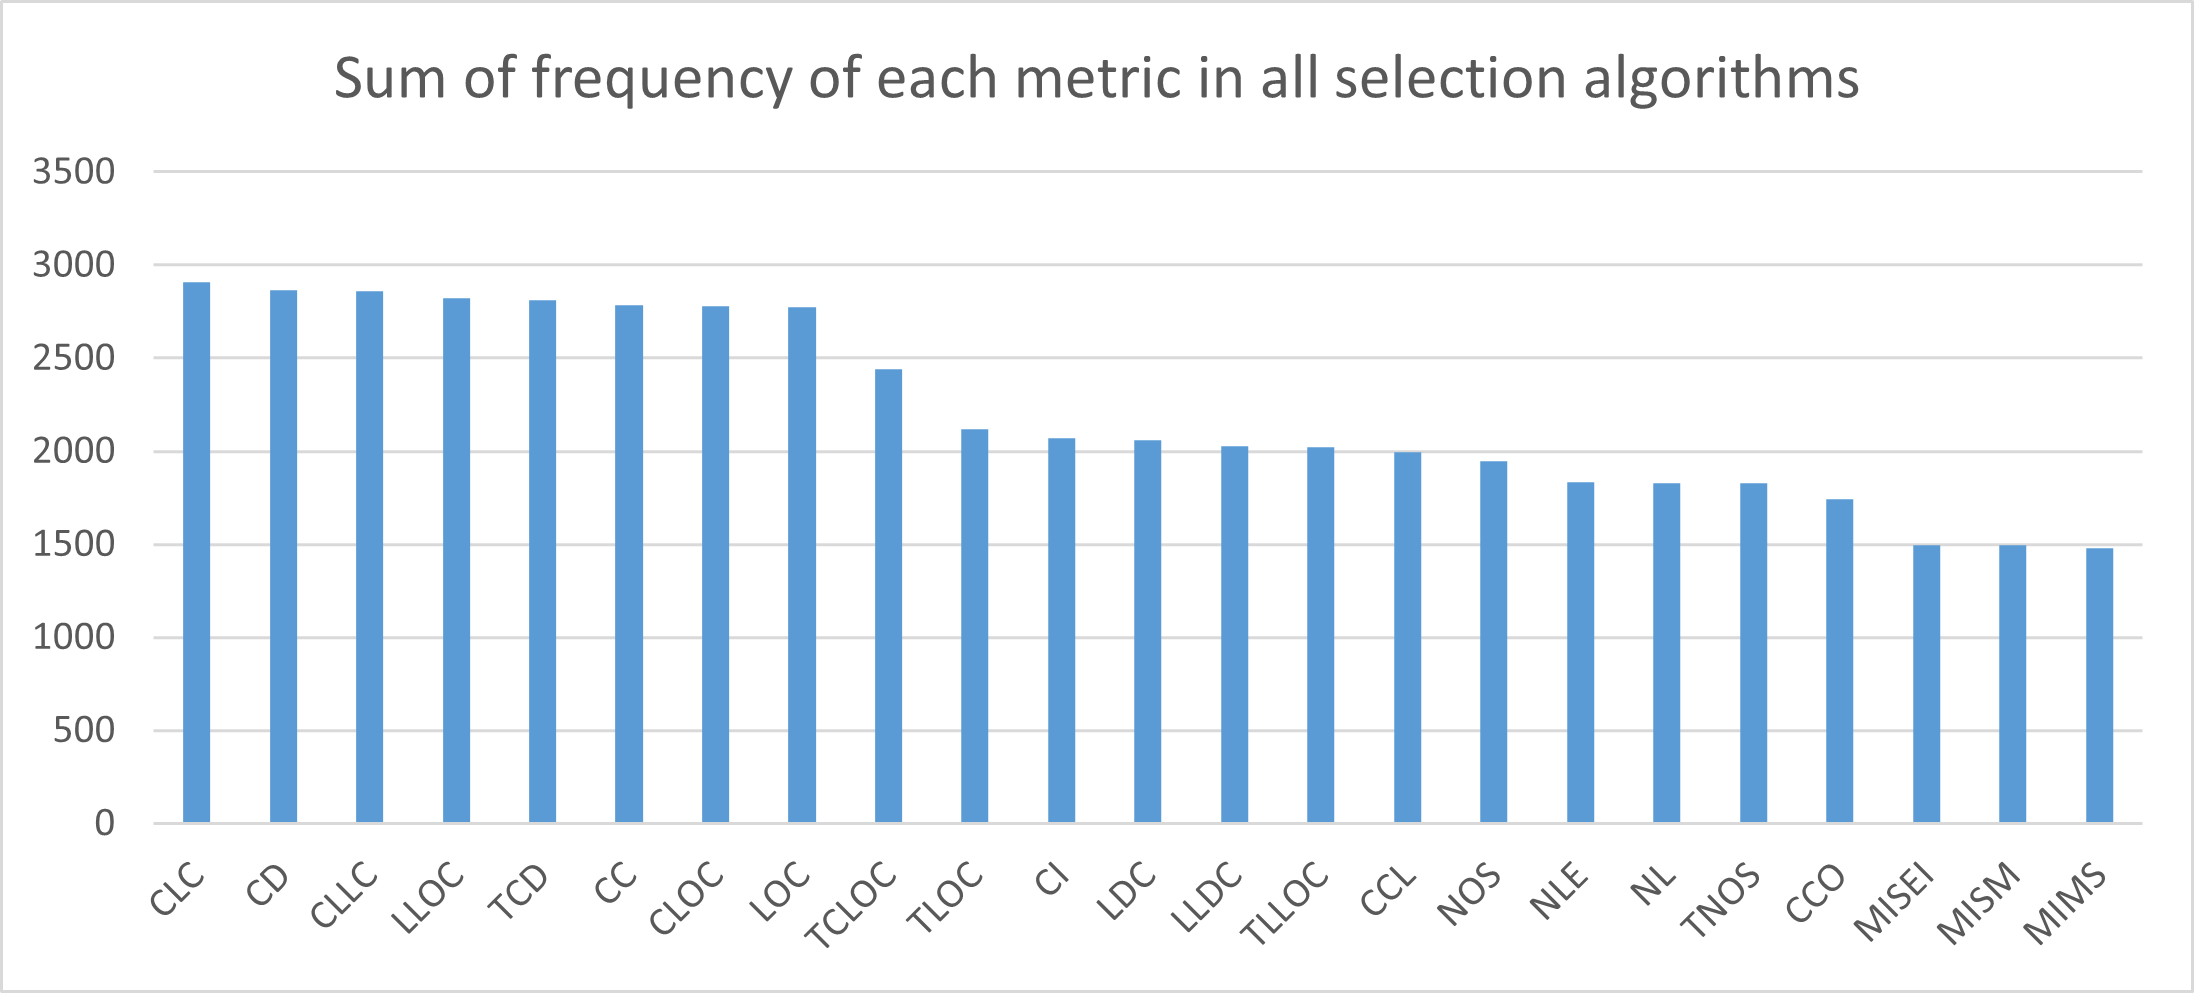
\includegraphics[width=0.95\columnwidth]{frec_all.png}
\caption{Frecuencia de selección de las métricas de código a través de los seis esquemas de selección de características.}
\label{fig:frecuencia}
\end{figure}

\textit{Advertencia sobre un posible artefacto de conteo.} Una explicación alternativa, no excluyente, para la alta frecuencia de selección de CLOC, LOC y LLOC es un artefacto de conteo: al ser las únicas tres métricas disponibles en los tres niveles de granularidad, tienen estructuralmente el triple de oportunidades de ser seleccionadas que una métrica exclusiva de un solo nivel, y el doble que una disponible en dos niveles. Los datos actuales no permiten distinguir, sin reprocesar los registros de selección del Paso 1 normalizando por nivel de granularidad, entre valor predictivo genuino y este efecto de oportunidad; esta verificación se declara como trabajo futuro (Sección \ref{sec:conclusiones}) y se documenta como amenaza a la validez de constructo en la Sección \ref{sec:amenazas}.

\subsection{RQ3: sensibilidad a los parámetros}

Sobre las 13.916 ejecuciones, la \textit{F-measure} promedió 0,547 (\textit{DE} = 0,104; mín. = 0,274; máx. = 0,844). La correlación entre \textit{F-measure} y \textit{Rank} fue de $-0{,}021$, entre \textit{F-measure} y $\beta$ de $0{,}027$, y entre \textit{Rank} y $\beta$ de $0{,}011$: en ninguno de los tres casos existe una asociación lineal relevante. No obstante, se observó una tendencia, sin llegar a ser una correlación fuerte, a obtener mejores valores de \textit{F-measure} con valores de \textit{Rank} más bajos y de $\beta$ más altos, mientras que en todos los casos las métricas seleccionadas redujeron sustancialmente el número de entradas del clasificador sin deteriorar su desempeño frente a la línea base.

\subsection{RQ4: efecto del balanceo de clases}
\label{sec:RQ4}

La Tabla \ref{tab:balance} resume la \textit{F-measure} promedio de las 13.916 ejecuciones agrupadas por técnica de balanceo, comparando el conjunto de entrenamiento original con su versión balanceada (el conjunto de prueba nunca se balancea). En los tres algoritmos, balancear el conjunto de entrenamiento no mejoró la \textit{F-measure} promedio respecto a entrenar con la distribución original; el efecto fue más marcado en RUS, cuya reducción de instancias de la clase mayoritaria disminuyó la cantidad de información disponible para el entrenamiento.

\begin{table}[H]
\caption{F-measure promedio según técnica de balanceo}
\label{tab:balance}
\centering
\begin{tabular}{lccc}
\toprule
Técnica & Sin balancear & Balanceado & $\Delta$ \\
\midrule
ROS   & 0,555 & 0,548 & $-0,007$ \\
RUS   & 0,555 & 0,524 & $-0,031$ \\
SMOTE & 0,555 & 0,548 & $-0,007$ \\
\bottomrule
\end{tabular}
\end{table}

Este resultado sugiere que, cuando el conjunto de prueba conserva la proporción real de clases del dominio, balancear artificialmente solo el entrenamiento no se traduce en una mejora del \textit{F-measure} promedio medido en condiciones realistas, incluso si estas técnicas suelen recomendarse para evitar el sesgo del clasificador hacia la clase mayoritaria.

Para contrastar formalmente esta observación se aplicó una prueba de Wilcoxon de rangos con signo, pareada por conjunto de datos, sobre el mejor \textit{F-measure} balanceado frente al mejor sin balancear de cada uno de los 16 conjuntos por nivel (los valores por proyecto corresponden a las Tablas \ref{tab:oryx} y \ref{tab:agg}). A nivel de método la diferencia resultó estadísticamente significativa a favor de la versión sin balancear ($p = 0{,}012$), aunque con un tamaño de efecto insignificante (Cliff's $\delta = 0{,}07$); a nivel de clase ($p = 0{,}48$) y de archivo ($p = 0{,}86$) no se detectaron diferencias significativas, y al agrupar los tres niveles el resultado quedó en el límite de la significancia ($p = 0{,}052$). En los cuatro casos el tamaño de efecto fue insignificante ($|\delta| < 0{,}15$).

Estas cifras deben interpretarse con cautela: las medias de la Tabla \ref{tab:balance} se analizaron de forma descriptiva sobre todas las ejecuciones, mientras que la prueba estadística se aplicó a la mejor configuración por proyecto, sujeta a un sesgo de selección optimista. Además, el \textit{F-measure} agregado pondera ambas clases por su frecuencia, de modo que la contribución de la clase de interés práctico (bug) queda diluida. Este efecto está acotado por el desequilibrio moderado de BugHunter (Tabla \ref{tab:desbalance}): con medianas de entre el 28,1\,\% y el 42,7\,\% de instancias \textit{bug} según el nivel, la clase minoritaria conserva un peso sustancial en la métrica agregada, muy por encima del que tendría en conjuntos con menos del 10\,\% de instancias defectuosas. Aun así, un análisis desagregado por la clase \textit{bug} ---no recuperable desde los resultados almacenados (Sección \ref{sec:diseno})--- podría matizar la conclusión, especialmente en los proyectos más desequilibrados como \textit{oryx} o \textit{antlr4}. La línea base del conjunto ``All'' a nivel de método (Tabla \ref{tab:porclase}) ilustra la magnitud del riesgo: un \textit{F-measure} ponderado de 0,565 convive con un \textit{F-measure} de 0,356 para la clase \textit{bug} y un MCC cercano a cero. El análisis de sensibilidad (Sección \ref{sec:sensibilidad}), que almacena métricas por clase para sus 28.440 ejecuciones, resuelve la pregunta que estos datos agregados dejaban abierta: el balanceo sí mejora de forma consistente el \textit{F-measure} de la clase \textit{bug} y el MCC en los tres clasificadores evaluados, aun cuando el \textit{F-measure} ponderado apenas varía. En conjunto, la evidencia indica que balancear solo el entrenamiento no mejora el \textit{F-measure} ponderado cuando el conjunto de prueba conserva la distribución real de clases ---coherente con un desequilibrio comparativamente leve---, pero sí desplaza el desempeño hacia la clase de interés práctico; la conclusión de RQ4 debe leerse, por tanto, condicionada a la métrica empleada.

\subsection{RQ5: proyecto unificado vs. proyectos individuales}

El conjunto ``All'', unión de los 15 proyectos en cada nivel, contiene considerablemente más instancias que cualquier proyecto individual, pero en ningún escenario (línea base, selección de características o balanceo de clases) obtuvo el mejor resultado de \textit{F-measure}; tampoco fue, en general, el peor. Este patrón se mantuvo de forma consistente en los tres niveles de granularidad. La evidencia sugiere que mezclar métricas de código de proyectos con metodologías de desarrollo, dominios y equipos distintos no mejora necesariamente la capacidad predictiva de los clasificadores, y que entrenar modelos específicos por proyecto resulta más efectivo que ampliar el volumen de datos combinando múltiples proyectos heterogéneos. Esta comparación se enmarca en la distinción clásica entre predicción de fallas intra-proyecto (\textit{Within-Project Defect Prediction}, WPDP) y entre proyectos (\textit{Cross-Project Defect Prediction}, CPDP), donde entrenar con datos de proyectos ajenos suele degradar el rendimiento por la heterogeneidad de las distribuciones \cite{cheng2022,sharma2023far}. Nuestro conjunto ``All'' constituye un escenario mixto, y su desempeño no superior a los proyectos individuales es coherente con lo reportado en esa línea de trabajo.

\subsection{Análisis de sensibilidad: clasificadores adicionales y línea base unificada}
\label{sec:sensibilidad}

El análisis de sensibilidad descrito en la Sección \ref{sec:diseno} responde dos preguntas: si la línea base es comparable cuando se elimina la diferencia de herramienta y esquema de validación, y si los hallazgos anteriores son específicos de Random Forest.

\textit{Línea base unificada.} Recalculada con RF bajo el mismo esquema \textit{holdout} estratificado 67/33 de \textit{scikit-learn} (todas las características, sin balanceo), la línea base promedia 0,62 a nivel de método, 0,52 a nivel de clase y 0,52 a nivel de archivo, frente a 0,63, 0,50 y 0,50 de la línea base Weka con validación cruzada (Tabla \ref{tab:baseline}). Las diferencias, de a lo sumo 0,02, indican que el factor de confusión introducido por el cambio de herramienta y esquema de validación no altera las conclusiones. En el conjunto ``All'' a nivel de método, además, el desglose por clase de esta línea base (\textit{F-measure} de la clase bug de 0,360; MCC de 0,069; AUC-ROC de 0,546) coincide estrechamente con el obtenido en Weka (Tabla \ref{tab:porclase}), corroborando ambas mediciones de forma independiente.

\textit{Generalización entre clasificadores.} La Tabla \ref{tab:sensibilidad} resume las diferencias pareadas sobre los 15 proyectos individuales. Tres patrones emergen. Primero, la selección de características no solo conserva, sino que \textit{mejora} el \textit{F-measure} ponderado en los tres clasificadores (mediana de $+0{,}001$ a $+0{,}041$, con mejora en 14 o 15 de los 15 proyectos y $p<0{,}01$ en todos los casos), con reducciones medianas de características de entre el 31\,\% y el 82\,\%: el hallazgo de RQ1 no es específico de RF. Segundo, el efecto del balanceo depende del clasificador y, sobre todo, de la métrica: en el \textit{F-measure} ponderado el balanceo no aporta en RF (consistente con RQ4), aporta marginalmente en XGBoost y mejora de forma significativa en la SVM lineal; pero en las métricas por clase el balanceo mejora la detección de la clase \textit{bug} de manera consistente en los \textit{tres} clasificadores (\textit{F-measure} de la clase bug: mediana de $+0{,}031$ a $+0{,}317$, con mejora en 12 a 15 de los 15 proyectos y $p<0{,}05$; MCC: mediana de $+0{,}013$ a $+0{,}055$). Es decir, el resultado nulo de RQ4 es en gran medida un artefacto de la métrica agregada: balancear el entrenamiento sí mejora la capacidad del modelo para identificar código defectuoso, a costa de la clase mayoritaria, y ese intercambio queda oculto en el \textit{F-measure} ponderado. Tercero, el conjunto ``All'' no obtuvo el mejor resultado en ningún clasificador ni nivel (puestos 7 a 15 de 16 en \textit{F-measure} ponderado; 6 a 13 de 16 en MCC), por lo que la conclusión de RQ5 también se generaliza, incluso bajo métricas insensibles al desequilibrio. Las diferencias globales entre clasificadores fueron pequeñas en magnitud (mediana pareada $\leq 0{,}023$ en el mejor \textit{F-measure} ponderado, a favor de la SVM lineal y XGBoost sobre RF), aunque la SVM lineal sin balanceo tiende fuertemente a la clase mayoritaria (mediana de \textit{F-measure} de la clase bug de 0,143 a nivel de método), lo que refuerza la necesidad de leer las métricas por clase junto al agregado. Ninguno de los tres clasificadores fue ajustado mediante búsqueda de hiperparámetros; la Sección \ref{sec:amenazas} discute la implicancia de esta decisión, en particular para la ganancia observada en la SVM lineal.

\begin{table}[H]
\caption{Análisis de sensibilidad por clasificador: mediana de las diferencias pareadas sobre los 15 proyectos (sel. = mejor esquema de selección vs. todas las características; bal. = mejor entrenamiento balanceado vs. sin balancear) y puesto de ``All'' entre los 16 conjuntos por mejor \textit{F-measure} ponderado}
\label{tab:sensibilidad}
\centering
\resizebox{\columnwidth}{!}{%
\begin{tabular}{llccccc}
\toprule
Clf. & Nivel & $\Delta F$ sel. & $\Delta F$ bal. & $\Delta F_{1}$ bug bal. & $\Delta$MCC bal. & ``All'' \\
\midrule
RF  & Método  & +0,014 & $-0,001$ & +0,108 & +0,036 & 9/16 \\
RF  & Clase   & +0,028 & +0,002   & +0,072 & +0,026 & 12/16 \\
RF  & Archivo & +0,033 & +0,011   & +0,040 & +0,021 & 12/16 \\
XGB & Método  & +0,014 & +0,005   & +0,135 & +0,045 & 11/16 \\
XGB & Clase   & +0,031 & +0,004   & +0,066 & +0,025 & 7/16 \\
XGB & Archivo & +0,041 & +0,012   & +0,031 & +0,027 & 7/16 \\
SVM & Método  & +0,006 & +0,024   & +0,317 & +0,055 & 15/16 \\
SVM & Clase   & +0,018 & +0,009   & +0,155 & +0,013 & 13/16 \\
SVM & Archivo & +0,001 & +0,033   & +0,206 & +0,041 & 13/16 \\
\bottomrule
\end{tabular}}
\end{table}

\section{Discusión}

Los resultados muestran que la selección de características en dos etapas es la técnica de preprocesamiento con mayor impacto práctico en este estudio en términos de reducción de dimensionalidad: reduce la mediana del número de métricas de BugHunter entre un 40\,\% y un 88\,\% según el nivel de granularidad (hasta un 94\,\% en el mejor caso individual) con una pérdida marginal de \textit{F-measure} inferior a 0,02, e incluso mejorándola levemente a nivel de archivo. En cambio, el balanceo de clases sobre el conjunto de entrenamiento no mejoró el \textit{F-measure} ponderado cuando el conjunto de prueba conserva la distribución real de clases; el análisis de sensibilidad muestra, sin embargo, que esta lectura depende de la métrica y del clasificador: en \textit{F-measure} de la clase \textit{bug} y en MCC el balanceo aporta mejoras consistentes en RF, XGBoost y SVM lineal (Sección \ref{sec:sensibilidad}). Esto reconcilia parcialmente nuestros resultados con la literatura que reporta beneficios del balanceo \cite{tantithamthavorn2020,rathi2023}: el beneficio existe, y no es menor: se concentra en la clase minoritaria y queda diluido ---o incluso invertido--- en la métrica agregada. La estabilidad de los hallazgos de RQ1 y RQ5 en los tres clasificadores indica, además, que no son artefactos del clasificador elegido. Asimismo, la consistencia de CLOC, LOC y LLOC como predictoras en los tres niveles refuerza hallazgos previos sobre el valor de las métricas de tamaño de código frente a métricas más complejas de acoplamiento o cohesión \cite{radjenovic2013}; si bien, como se discute en la Sección \ref{sec:RQ2}, esta consistencia debe leerse con cautela dado que estas tres métricas cuentan estructuralmente con más oportunidades de selección, y el hecho de que un proyecto unificado no supere a los proyectos individuales confirma que la heterogeneidad entre proyectos de software limita el valor de combinar datasets sin un tratamiento adicional de dominio.

\subsection{Amenazas a la validez}
\label{sec:amenazas}

Respecto a la \textbf{validez de constructo}, en el estudio principal el \textit{F-measure} se reporta como valor agregado ponderado por la frecuencia de clase y no se desagrega por la clase minoritaria (bug); dado que en conjuntos desequilibrados la métrica agregada tiende a estar dominada por la clase mayoritaria, la interpretación de los resultados de RQ4 podría variar bajo una métrica específica de la clase de interés ---y de hecho varía, como muestra el análisis por clase de la Sección \ref{sec:sensibilidad}---. La magnitud de este sesgo está acotada por el desequilibrio moderado del conjunto de datos (Tabla \ref{tab:desbalance}), pero no es despreciable en los proyectos más desequilibrados, donde el valor agregado puede sobrestimar la utilidad práctica del modelo para detectar código defectuoso. A ello se suma una \textbf{limitación de reproducibilidad} que se declara explícitamente: de cada una de las 13.916 ejecuciones originales se almacenaron solo las métricas agregadas (Sección \ref{sec:diseno}), sin predicciones individuales, matrices de confusión ni probabilidades estimadas, por lo que sus métricas por clase no pueden recomputarse sin repetirlas. Esta limitación queda acotada por dos vías: la línea base Weka del conjunto ``All'' a nivel de método (Tabla \ref{tab:porclase}) y, sobre todo, el análisis de sensibilidad (Sección \ref{sec:sensibilidad}), que almacena el \textit{F-measure} de la clase \textit{bug}, el MCC y el AUC-ROC para la totalidad de sus 28.440 ejecuciones y cuyo desglose por clase modifica sustantivamente la lectura de RQ4.

Una segunda amenaza de constructo, no discutida en la versión original, concierne a RQ2: la mayor frecuencia de selección observada para CLOC, LOC y LLOC (Fig.~\ref{fig:frecuencia}) podría reflejar, al menos parcialmente, que estas son las únicas métricas presentes en los tres niveles de granularidad y, por tanto, cuentan con más oportunidades estructurales de ser seleccionadas que las métricas exclusivas de un nivel. Distinguir esta explicación de un valor predictivo genuino exige normalizar la frecuencia de selección por el número de oportunidades, lo cual se declara como trabajo futuro (Sección \ref{sec:conclusiones}).

En cuanto a la \textbf{validez de conclusión}, el efecto del balanceo se contrastó con una prueba de Wilcoxon de rangos con signo pareada y con tamaños de efecto (Cliff's $\delta$) sobre la mejor configuración por proyecto (Sección \ref{sec:RQ4}); no obstante, las medias sobre la totalidad de las 13.916 ejecuciones se analizaron únicamente de forma descriptiva y la comparación pareada se basa en configuraciones seleccionadas post-hoc, por lo que una validación cruzada repetida junto con pruebas ómnibus (por ejemplo, Scott-Knott ESD) reforzaría estas conclusiones. Esta misma amenaza, i.e., comparar el máximo sobre un conjunto de configuraciones frente a una única configuración de referencia, afecta también a RQ1 (Tablas \ref{tab:oryx} y \ref{tab:sensibilidad}), donde el mejor esquema de selección se compara contra la única configuración de ``todas las características''; a diferencia de RQ4, donde ambos brazos de la comparación maximizan sobre la misma malla de configuraciones y el sesgo tiende a cancelarse, en RQ1 la asimetría no se cancela. Por ello, la Sección \ref{sec:RQ1} apoya su conclusión principal en las medianas de las Tablas \ref{tab:agg} y \ref{tab:sensibilidad} en lugar de en el máximo individual de 94\,\%.

Sobre la \textbf{validez interna}, la línea base original se calculó en Weka con validación cruzada de 10 particiones, mientras que los experimentos de selección de características y balanceo emplearon \textit{scikit-learn} con un esquema \textit{holdout} estratificado 67/33, un factor de confusión que limitaba la comparación directa; esta amenaza se mitigó recalculando la línea base bajo el mismo esquema y herramienta de los experimentos (Sección \ref{sec:sensibilidad}), con diferencias de a lo sumo 0,02 respecto de la versión Weka, por lo que su impacto sobre las conclusiones es menor. Una segunda amenaza a la validez interna, no discutida en la versión original, es que el análisis de relevancia y redundancia (Sección \ref{sec:seleccion}) se calcula sobre el conjunto proyecto-nivel completo, antes de la partición entrenamiento/prueba, mientras que el balanceo de clases sí se aplica exclusivamente sobre el conjunto de entrenamiento (Sección \ref{sec:balanceo}). Dado que los algoritmos de relevancia utilizan la etiqueta de clase, este diseño introduce un riesgo de sesgo de selección sobre el subconjunto de características elegido, en línea con lo documentado por Ambroise y McLachlan \cite{ambroise2002} y por Cawley y Talbot \cite{cawley2010} para esquemas de selección no anidados en validación cruzada. Dicho riesgo no afecta el ajuste de los parámetros del clasificador, realizado exclusivamente sobre el conjunto de entrenamiento resultante, pero sí puede inflar de forma optimista la comparación entre ``todas las características'' y el mejor esquema de selección reportada en RQ1. Adicionalmente, ninguno de los tres clasificadores fue ajustado mediante búsqueda de hiperparámetros; en particular, la ganancia de \textit{F-measure} de la clase \textit{bug} de hasta $+0{,}317$ observada para la SVM lineal en el análisis de sensibilidad (Tabla \ref{tab:sensibilidad}) podría estar sobrestimada respecto de una SVM con hiperparámetros ajustados que exhibiera, sin balanceo, un sesgo menor hacia la clase mayoritaria.

Finalmente, respecto a la \textbf{validez externa}, el estudio principal se limita a Random Forest; el análisis de sensibilidad la mitiga parcialmente al replicar los hallazgos con XGBoost y una SVM lineal ---dos paradigmas distintos---, aunque persisten las restantes acotaciones: 15 proyectos Java, una malla de parámetros discreta ($\{0{,}5, 0{,}7, 0{,}9\}$ para \textit{Rank} y $\beta$), una única partición 67/33 con semilla fija tanto en el estudio principal como en el análisis de sensibilidad (Sección \ref{sec:diseno}) y familias de clasificadores no cubiertas (por ejemplo, redes neuronales), por lo que los hallazgos podrían no generalizarse directamente a otros lenguajes o configuraciones más finas.

\section{Conclusiones y Trabajo Futuro}
\label{sec:conclusiones}

El resultado más relevante es que el efecto del balanceo de clases sobre el entrenamiento depende críticamente de la métrica de evaluación: aplicado solo al conjunto de entrenamiento, el balanceo no mejora el \textit{F-measure} ponderado cuando el conjunto de prueba conserva la distribución real de clases ---resultado confirmado por una prueba de Wilcoxon pareada con tamaño de efecto insignificante ($|\delta| < 0{,}15$) en los tres niveles de granularidad---, pero sí mejora de forma consistente la detección de la clase minoritaria (mediana de $+0{,}031$ a $+0{,}317$ en \textit{F-measure} de la clase \textit{bug}, y $+0{,}013$ a $+0{,}055$ en MCC) en Random Forest, XGBoost y SVM lineal. Esta discrepancia entre la métrica agregada y las métricas por clase ilustra un riesgo metodológico frecuente en dominios con desequilibrio moderado: un \textit{F-measure} ponderado aceptable puede coexistir con una detección casi nula de la clase de interés práctico.

A partir de las limitaciones declaradas del estudio (Secciones \ref{sec:metodologia} y \ref{sec:amenazas}), y la retroalimentación recibida en el proceso de revisión, se identifican las siguientes extensiones para el trabajo futuro:

\begin{itemize}
\item \textbf{Selección de características anidada.} Recalcular la selección de características de forma anidada, exclusivamente dentro de cada partición de entrenamiento, para eliminar el riesgo de sesgo de selección identificado en la Sección \ref{sec:amenazas} \cite{ambroise2002,cawley2010}; esto exige reejecutar la totalidad de las 13.916 y 28.440 ejecuciones.
\item \textbf{Validación cruzada repetida en el estudio principal.} Repetir el estudio de 13.916 ejecuciones bajo un esquema de validación cruzada repetida, sin una semilla única, junto con pruebas ómnibus (Scott-Knott ESD), extendiendo al estudio principal la mejora ya prevista originalmente solo para el análisis de sensibilidad.
\item \textbf{Reanálisis de RQ2 normalizado por oportunidades.} Reprocesar los registros de selección de características del Paso 1, normalizando la frecuencia de selección de cada métrica por su número de oportunidades (niveles de granularidad en que está disponible) o reportando un ranking independiente por nivel, para distinguir el valor predictivo genuino de CLOC, LOC y LLOC del artefacto de conteo señalado en la Sección \ref{sec:RQ2}.
\item \textbf{Ajuste de hiperparámetros.} Incorporar búsqueda de hiperparámetros para Random Forest, XGBoost y, en particular, la SVM lineal, antes de atribuir a la técnica de balanceo la mejora observada en la detección de la clase \textit{bug} (Tabla \ref{tab:sensibilidad}).
\item \textbf{Reestructuración para una versión de revista.} Producir una versión extendida en la que el análisis de sensibilidad con métricas por clase (Sección \ref{sec:sensibilidad}) constituya la evidencia primaria, y el estudio de 13.916 ejecuciones se reporte como el estudio exploratorio inicial que lo motivó.
\item \textbf{Replicación en otros lenguajes y niveles de desequilibrio.} Replicar la metodología sobre proyectos en otros lenguajes (Python, C++) y sobre conjuntos con desequilibrio más severo (por ejemplo, proyectos NASA con $<$10\,\% de instancias defectuosas), para determinar si los hallazgos se sostienen más allá de BugHunter.
\item \textbf{Integración de modelos de lenguaje de gran escala.} Evaluar la integración de representaciones basadas en LLM \cite{hou2024,fan2023} como fuente complementaria a las métricas estáticas seleccionadas, para determinar si aportan mejoras reales sobre la línea base tabular establecida en este trabajo, a un costo computacional justificado.
\end{itemize}

\section*{Disponibilidad de Datos y Reproducibilidad}
El conjunto de datos BugHunter empleado en este estudio es de acceso público \cite{ferenc2020}. Los conjuntos de datos procesados, los \textit{scripts} de selección de características y balanceo, y los resultados de las 13.916 ejecuciones están disponibles a solicitud de los autores. Dichos resultados contienen, por ejecución, las métricas agregadas (precisión, \textit{recall}, \textit{F-measure} y exactitud) y los parámetros de la configuración correspondiente, pero no las predicciones por instancia, por lo que no permiten derivar métricas por clase sin reejecutar los experimentos. La excepción es la salida completa de Weka de la línea base del conjunto ``All'' a nivel de método ---matriz de confusión y desglose por clase (Tabla \ref{tab:porclase})---, que también está disponible. Los resultados del análisis de sensibilidad (28.440 ejecuciones con RF, XGBoost y SVM lineal) se distribuyen íntegros junto con sus \textit{scripts}: cada registro incluye la configuración completa y las métricas agregadas y por clase (precisión, \textit{recall} y \textit{F-measure} de la clase \textit{bug}, MCC y AUC-ROC), lo que permite reproducir todos los análisis de la Sección \ref{sec:sensibilidad}.

\section*{Agradecimientos}
Los autores agradecen al proyecto ``Fortaleciendo la Investigación en Inteligencia Artificial y sus Aplicaciones'', código BIP 40067596-0, Fondo Regional para la Producción y Desarrollo, y GORE Antofagasta, por el apoyo para el desarrollo de esta investigación y la difusión de sus resultados.

\begin{thebibliography}{00}

\bibitem{singh2024} M. Singh and J. K. Chhabra, ``Improved software fault prediction using new code metrics and machine learning algorithms,'' \textit{Journal of Computer Languages}, vol. 78, p. 101253, 2024.

\bibitem{ferenc2020} R. Ferenc, P. Gyimesi, G. Gyimesi, Z. T{\'o}th, and T. Gyim{\'o}thy, ``An automatically created novel bug dataset and its validation in bug prediction,'' \textit{Journal of Systems and Software}, vol. 169, p. 110691, 2020.

\bibitem{promise2005} J. Sayyad Shirabad and T. J. Menzies, ``The PROMISE repository of software engineering databases,'' School of Information Technology and Engineering, University of Ottawa, Canada, 2005.

\bibitem{uci1987} ``UCI Machine Learning Repository.'' [Online]. Available: https://archive.ics.uci.edu/datasets

\bibitem{rathi2023} S. C. Rathi, S. Misra, R. Colomo-Palacios, R. Adarsh, L. B. M. Neti, and L. Kumar, ``Empirical evaluation of the performance of data sampling and feature selection techniques for software fault prediction,'' \textit{Expert Systems with Applications}, vol. 223, p. 119806, 2023.

\bibitem{tantithamthavorn2020} C. Tantithamthavorn, A. E. Hassan, and K. Matsumoto, ``The impact of class rebalancing techniques on the performance and interpretation of defect prediction models,'' \textit{IEEE Transactions on Software Engineering}, vol. 46, no. 11, pp. 1200--1219, 2020.

\bibitem{osa2004} ``OpenStaticAnalyzer,'' SED Inf. U-Szeged. [Online]. Available: https://github.com/sed-inf-u-szeged/OpenStaticAnalyzer

\bibitem{singh2021survey} M. R. O. Singh and B. Thankachan, ``A detailed survey on machine intelligence based frameworks for software defect prediction,'' in \textit{Proc. 2021 Int. Conf. Computing, Communication, and Intelligent Systems (ICCCIS)}, 2021, pp. 360--365.

\bibitem{li2018} Z. Li, X.-Y. Jing, and X. Zhu, ``Progress on approaches to software defect prediction,'' \textit{IET Software}, vol. 12, no. 3, pp. 161--175, 2018.

\bibitem{liu2015} W. Liu, S. Liu, Q. Gu, J. Chen, X. Chen, and D. Chen, ``Empirical studies of a two-stage data preprocessing approach for software fault prediction,'' \textit{IEEE Transactions on Reliability}, vol. 65, no. 1, pp. 38--53, 2016.

\bibitem{chen2013} J. Chen, S. Liu, X. Chen, Q. Gu, and D. Chen, ``Empirical studies on feature selection for software fault prediction,'' in \textit{Proc. 5th Asia-Pacific Symp. Internetware (Internetware '13)}, 2013.

\bibitem{yu2003} L. Yu and H. Liu, ``Feature selection for high-dimensional data: A fast correlation-based filter solution,'' in \textit{Proc. 20th Int. Conf. Machine Learning (ICML)}, 2003, pp. 856--863.

\bibitem{hossen2020} M. Hossen, M. Islam, N. Yusof, M. Rahman, F. Siddika, M. Rahman, S. Khatun, M. S. Abdul Karim, and S. M. H. Mahmud, ``Hybrid sampling and random forest based machine learning approach for software defect prediction,'' in \textit{Advances in Intelligent Systems and Computing}. Springer, 2020, pp. 541--553.

\bibitem{sikic2022} L. {\v S}iki\'c, A. S. Kurdija, K. Vladimir, and M. {\v S}ili\'c, ``Graph neural network for source code defect prediction,'' \textit{IEEE Access}, vol. 10, pp. 10402--10415, 2022.

\bibitem{zhou2022} C. Zhou, P. He, C. Zeng, and J. Ma, ``Software defect prediction with semantic and structural information of codes based on graph neural networks,'' \textit{Information and Software Technology}, vol. 152, p. 107057, 2022.

\bibitem{liu2024sedpgk} W. Liu, Y. Yue, X. Chen, Q. Gu, P. Zhao, X. Liu, and J. Zhao, ``SeDPGK: Semi-supervised software defect prediction with graph representation learning and knowledge distillation,'' \textit{Information and Software Technology}, vol. 174, p. 107510, 2024.

\bibitem{pornprasit2023} C. Pornprasit and C. Tantithamthavorn, ``DeepLineDP: Towards a deep learning approach for line-level defect prediction,'' \textit{IEEE Transactions on Software Engineering}, vol. 49, no. 1, pp. 84--98, 2023.

\bibitem{jiang2024} S. Jiang, Y. Chen, Z. He \textit{et al.}, ``Cross-project defect prediction via semantic and syntactic encoding,'' \textit{Empirical Software Engineering}, vol. 29, art. 80, 2024.   % <-- VERIFICAR lista completa de autores

\bibitem{guo2023} Y. Guo, X. Gao, Z. Zhang, W. K. Chan, and B. Jiang, ``A study on the impact of pre-trained model on just-in-time defect prediction,'' in \textit{Proc. IEEE 23rd Int. Conf. Software Quality, Reliability, and Security (QRS)}, 2023.   % <-- VERIFICAR páginas

\bibitem{nam2026} D. Nam, T. Kim, D. Ryu, and J. Baik, ``ReDef: Do code language models truly understand code changes for just-in-time software defect prediction?'' \textit{Proceedings of the ACM on Software Engineering} (FSE 2026), 2026.   % <-- VERIFICAR volumen/número de artículo

\bibitem{giray2023} G. Giray, K. E. Bennin, \"O. K\"oksal, \"O. Babur, and B. Tekinerdogan, ``On the use of deep learning in software defect prediction: A systematic literature review,'' \textit{Journal of Systems and Software}, vol. 195, p. 111537, 2023.

\bibitem{stradowski2023} S. Stradowski and L. Madeyski, ``Machine learning in software defect prediction: A business-driven systematic mapping study,'' \textit{Information and Software Technology}, vol. 155, p. 107128, 2023.

\bibitem{hou2024} X. Hou, Y. Zhao, Y. Liu, Z. Yang, K. Wang, L. Li, X. Luo, D. Lo, J. Grundy, and H. Wang, ``Large language models for software engineering: A systematic literature review,'' \textit{ACM Transactions on Software Engineering and Methodology}, vol. 33, no. 8, art. 220, 2024.

\bibitem{fan2023} A. Fan, B. Gokkaya, M. Harman, M. Lyubarskiy, S. Sengupta, S. Yoo, and J. M. Zhang, ``Large language models for software engineering: Survey and open problems,'' in \textit{Proc. IEEE/ACM Int. Conf. Software Engineering: Future of Software Engineering (ICSE-FoSE)}, 2023, pp. 31--53.

\bibitem{chen2026llm} Y. Chen, Y. Shen, T. Wang \textit{et al.}, ``Software defect detection using large language models: A literature review,'' \textit{Frontiers of Computer Science}, vol. 20, art. 2006202, 2026.   % <-- VERIFICAR lista completa de autores


\bibitem{junsomboon2017} N. Junsomboon and T. Phienthrakul, ``Combining over-sampling and under-sampling techniques for imbalance dataset,'' in \textit{Proc. 9th Int. Conf. Machine Learning and Computing}, 2017, pp. 243--247.

\bibitem{shah2020} K. Shah, H. Patel, D. Sanghvi, and M. Shah, ``A comparative analysis of logistic regression, random forest and KNN models for the text classification,'' \textit{Augmented Human Research}, vol. 5, no. 1, p. 12, 2020.

\bibitem{weka2005} I. H. Witten and E. Frank, \textit{Data Mining: Practical Machine Learning Tools and Techniques}, 2nd ed. San Francisco, CA: Morgan Kaufmann, 2005.

\bibitem{chen2016} T. Chen and C. Guestrin, ``XGBoost: A scalable tree boosting system,'' in \textit{Proc. 22nd ACM SIGKDD Int. Conf. Knowledge Discovery and Data Mining}, 2016, pp. 785--794.

\bibitem{cortes1995} C. Cortes and V. Vapnik, ``Support-vector networks,'' \textit{Machine Learning}, vol. 20, no. 3, pp. 273--297, 1995.

\bibitem{cheng2022} T. Cheng, K. Zhao, S. Sun, M. Mateen, and J. Wen, ``Effort-aware cross-project just-in-time defect prediction framework for mobile apps,'' \textit{Frontiers of Computer Science}, vol. 16, no. 6, art. 166207, 2022.

\bibitem{sharma2023far} U. Sharma and R. Sadam, ``How far does the predictive decision impact the software project? The cost, service time, and failure analysis from a cross-project defect prediction model,'' \textit{Journal of Systems and Software}, vol. 195, p. 111522, 2023.

\bibitem{radjenovic2013} D. Radjenovi{\'c}, M. Heri{\v c}ko, R. Torkar, and A. {\v Z}ivkovi{\v c}, ``Software fault prediction metrics: A systematic literature review,'' \textit{Information and Software Technology}, vol. 55, no. 8, pp. 1397--1418, 2013.

\bibitem{ambroise2002} C. Ambroise and G. J. McLachlan, ``Selection bias in gene extraction on the basis of microarray gene-expression data,'' \textit{Proceedings of the National Academy of Sciences}, vol. 99, no. 10, pp. 6562--6566, 2002.

\bibitem{cawley2010} G. C. Cawley and N. L. C. Talbot, ``On over-fitting in model selection and subsequent selection bias in performance evaluation,'' \textit{Journal of Machine Learning Research}, vol. 11, no. 70, pp. 2079--2107, 2010.

\end{thebibliography}

\end{document}
